\chapter{Exceptions in programming languages}

``Exceptions'' is a broader term referring to a strategy of handling erroneous
states in computer programs by interrupting normal program execution, running special
code called an \emph{exception handler} and then resuming execution in a known, different
state.

The usual terminology is not very strict: the word ``exception'' may mean sligtly
different things -- or different sides of the same thing -- in different contexts.
For example, programming languages are said to \emph{have exceptions} if they support
this kind of error handling; exceptions are said to \emph{be compiled}, while it is the
corresponding infrastructure and support code that is compiled; often the word ``exception''
denotes a piece of information about the error being handled; et cetera.

When an error occurs during normal execution of a program, \emph{an exception is thrown}%
\footnote{Some programming languages, such as Python, use the term \emph{raised}.%
\cite{python:reference}}.
This starts the
process of \emph{handling the exception}: looking for a suitable
\emph{exception handler} that \emph{handles the exception}, either by \emph{catching} it
to resume normal computation, or by \emph{re-throwing} it to find another handler
able to deal with the error.

Due to common names of the corresponding syntactic features of popular programming languages%
\footnote{Most of them use the same keywords for this purpose.},
a piece of code together with attached pieces of handler code is called a \emph{try-block},
and a piece of handler code is called a \emph{catch-block}.

Most languages also provide \emph{finally-blocks}. These are pieces of code attached to a
try-block that are guaranteed to be executed after the try-block, whether an exception
has been thrown or not. Because of this property, finally-blocks are usually used to clean up
resources. In this thesis, we will not model finally-blocks as these can be
supplemented by an appropriate use of all-catching exception handlers.

There may be multiple handlers attached to a piece of code.
As already mentioned, the word ``exception'' also denotes a piece of information about
the error or condition causing the exceptional state, modeled by a value of the programming
language. In typed languages, these values have types, exception handlers declare what
types of exceptions they can handle, and based on the type of the thrown exception,
an appropriate handler is selected. The handler can then inspect the exception and
behave appropriately.

A try-block needn't have handlers for all exceptions that might arise within. If an exception
is \emph{uncaught} within a try-block, it is \emph{propagated} to the containing try-block,
which may not catch this exception as well, propagating it further.
If an exception propagates all the way out of all nested try-blocks, the program usually
aborts.

To give a quick illustration how try-blocks look in the concrete syntax of some widely used
languages, \Fref{fig:try-blocks} contains four examples.\footnote{Note that OCaml does not
have syntax for finally-blocks; these are simulated by a function. Haskell does not have
syntax for exceptions at all, both \emph{catch} and \emph{finally} are just functions.
All code snippets are just symbolic and have been stripped of non-relevant context, such
as library imports and the definitions of the functions \emph{perform\_work}
and \emph{do\_cleanup}.}

\begin{figure}
%
\begin{subfigure}[b]{0.46\textwidth}\begin{codepy}
try:
	perform_work()
except IOError:
	print "IO error caught"
finally:
	do_cleanup()
\end{codepy}\caption{Python}\end{subfigure}
%
\begin{subfigure}[b]{0.46\textwidth}\begin{codejava}
try {
	performWork();
} catch (IOException e) {
	System.out.println(
	    "IO error caught");
} finally {
	doCleanup();
}
\end{codejava}\caption{Java}\end{subfigure}

\begin{subfigure}[b]{0.46\textwidth}\begin{codehs}
performWork
 `catch` (\(e :: IOException) ->
   putStrLn "IO error caught")
 `finally` 
   doCleanup
\end{codehs}\caption{Haskell}\end{subfigure}
%
\begin{subfigure}[b]{0.46\textwidth}\begin{codeml}
finally do_cleanup (fun () ->
  try perform_work ()
  with IO_error ->
    print_string "IO error caught"
) ()
\end{codeml}\caption{OCaml}\end{subfigure}

\caption{Try-blocks in different languages}
\label{fig:try-blocks}
\end{figure}

\todo{Really include ``finally''? Revise OCaml.}

\section{Purpose}

As already mentioned, in practice, exceptions are mostly used to handle errors or
other exceptional states. The advantage to using
exceptions for this purpose is separation of concerns and hence cleaner resulting code.
Especially when reading a program, the reader first reads the code related the expected
execution path, uncluttered with error checks, which brings forward the main idea
of the code.

However, some languages, for example Python or OCaml, use exceptions also for control-flow
purposes, not only in rare critical events. Python iterators raise an exception to
indicate the end of stream \cite{python:reference}; also file-I/O functions in OCaml raise
an exception to indicate the end of file \cite{ocaml:reference}. The implementation of
exceptions in these languages is efficient enough to make them cheap and enable this approach.

\todo{Disadvantages. Multiple exit points, reasoning.}

\todo{Extend this section.}

\section{History}

Louden and Lambert describe the invention of exceptions in their book
\emph{Programming Languages: Principles and Practice} as follows.

\begin{quote}
Exception handling was pioneered by the language PL/I in the 1960s and
significantly advanced by CLU in the 1970s, with the major design questions
eventually resolved in the 1980s and early 1990s. Today, virtually all major
current languages, including C++, Java, Ada, Python, ML, and Common Lisp (but
not C, Scheme or Smalltalk) have built-in exception handling mechanisms.
Exception handling has, in particular, been integrated very well into
object-oriented mechanisms in Python, Java, and C++, and into functional
mechanisms in ML and Common Lisp. Also, languages that do not have built-in
mechanisms sometimes have libraries available that provide them, or have other
built-in ways of simulating them. \cite[p.~423]{louden:languages}
\end{quote}

% http://stackoverflow.com/questions/1449951/what-language-was-the-first-to-implement-exception-handling

\todo{Extend this section.}

\section{Theoretical appeal}

The theoretical appeal of exceptions in function languages is impossible to discuss
without having introduced the \emph{Curry-Howard correspondence}.

\subsection{The Curry-Howard correspondence}

The Curry-Howard correspondence establishes a relationship between typed programs and logic.
According to this interpretation, types of programs correspond to logical propositions --
and programs themselves correspond to proofs of logical propositions corresponding to their
types.

This correspondence goes all the way to relating whole $\lambda$-calculi to different
logical systems. For example, the simply typed $\lambda$-calculus corresponds to the minimal
logic, see \Fref{fig:stlc-ml}.

\begin{figure}
\centering
\begin{subfigure}[b]{0.45\textwidth}
\begin{prooftree}
\bax{$x : \sigma \in \Gamma$}
\bright{Ax}\bun{$\Gamma \vdash x : \sigma$}
\end{prooftree}
\begin{prooftree}
\bax{$\Gamma, x : \sigma \vdash M : \tau$}
\bright{Abstr}\bun{$\Gamma \vdash (\lambda x:\sigma. M) : \sigma \to \tau$}
\end{prooftree}
\begin{prooftree}
\bax{$\Gamma \vdash f : \sigma \to \tau$}
\bax{$\Gamma \vdash x : \sigma$}
\bright{App}\bbin{$\Gamma \vdash f x : \tau$}
\end{prooftree}

\caption{$\lambda_\to$}
\end{subfigure}
%
\begin{subfigure}[b]{0.45\textwidth}
\begin{prooftree}
\bax{$A \in \Gamma$}
\bright{Ax}\bun{$\Gamma \vdash A$}
\end{prooftree}
\begin{prooftree}
\bax{$\Gamma, A \vdash B$}
\bright{$I_\to$}\bun{$\Gamma \vdash A \to B$}
\end{prooftree}
\begin{prooftree}
\bax{$\Gamma \vdash A \to B$}
\bax{$\Gamma \vdash A$}
\bright{$E_\to$}\bbin{$\Gamma \vdash B$}
\end{prooftree}
\caption{$ML$}
\end{subfigure}

\caption{Simply typed $\lambda$-calculus ($\lambda_\to$), compared to minimal logic (ML).}
\label{fig:stlc-ml}
\end{figure}

When put side-by-side, it can be seen that the typing rules for the simply typed
$\lambda$-calculus become precisely the natural-deduction rules for minimal logic
if terms are erased and only types are retained.

In this interpretation, \emph{function application} on the computational side corresponds
to \emph{modus ponens} (or implication elimination) on the logic side, and
\emph{$\lambda$-abstraction} corresponds to the \emph{deduction theorem} (or implication
introduction).

The correspondence between certain $\lambda$-calculi and logic systems was presented
by Barendregt in \cite{barendregt91} in the elegant form of the $\lambda$-cube, as seen in
\Fref{fig:lambda-cube}. The names of the $\lambda$-calculi and the corresponding
logic systems are listed in \Fref{tab:lambda-cube}.

\begin{figure}
\centering
\begin{subfigure}{0.4\textwidth}
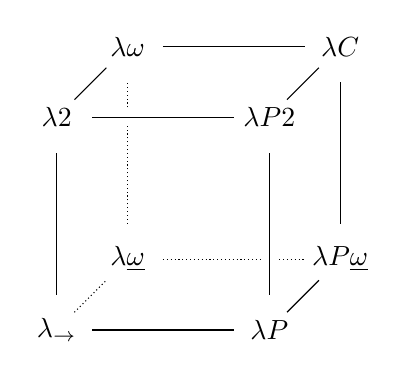
\begin{tikzpicture}[x=9mm,y=9mm,
        back line/.style={densely dotted,-},
        normal line/.style={-stealth,-},
        cross line/.style={normal line,-,
           preaction={draw=white, -, 
           line width=6pt}},
    ]
    \draw
    	(0,0) node{$\lambda_\to$}
    	(3,0) node{$\lambda{}P$}
    	(0,3) node{$\lambda{}2$}
    	(3,3) node{$\lambda{}P2$}
    	(1,1) node{$\lambda\underline{\omega}$}
    	(4,1) node{$\lambda{}P\underline{\omega}$}
    	(1,4) node{$\lambda\omega$}
    	(4,4) node{$\lambda{}C$}
	    ;
	\draw
		(1,1)
		+(0.5,0) edge[back line] +(2.5,0)
		+(0,0.5) edge[back line] +(0,2.5)
		+(0.5,3) edge[normal line] +(2.5,3)
		+(3,0.5) edge[normal line] +(3,2.5)
		;
	\draw[normal line]
		(0,0)
		+(0.5,0) edge +(2.5,0)
		+(0,0.5) edge +(0,2.5)
		+(0.5,3) edge[cross line] +(2.5,3)
		+(3,0.5) edge[cross line] +(3,2.5)
		;
	\draw
		(0,3) +(0.25,0.25) edge[normal line] +(0.7,0.7)
		(3,3) +(0.25,0.25) edge[normal line] +(0.7,0.7)
		(3,0) +(0.25,0.25) edge[normal line] +(0.7,0.7)
		(0,0) +(0.25,0.25) edge[back line] +(0.7,0.7)
		;
\end{tikzpicture}
\caption{$\lambda$-cube}
\end{subfigure}
%
\begin{subfigure}{0.4\textwidth}
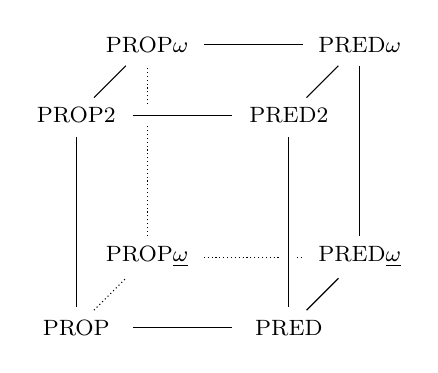
\begin{tikzpicture}[x=9mm,y=9mm,
        back line/.style={densely dotted,-},
        normal line/.style={-stealth,-},
        cross line/.style={normal line,-,
           preaction={draw=white, -, 
           line width=6pt}},
    ]
    \draw[font=\footnotesize]
    	(0,0) node{PROP}
    	(3,0) node{PRED}
    	(0,3) node{PROP2}
    	(3,3) node{PRED2}
    	(1,1) node{PROP$\underline{\omega}$}
    	(4,1) node{PRED$\underline{\omega}$}
    	(1,4) node{PROP$\omega$}
    	(4,4) node{PRED$\omega$}
	    ;
	\draw
		(1,1)
		+(0.8,0) edge[back line] +(2.2,0)
		+(0,0.3) edge[back line] +(0,2.7)
		+(0.8,3) edge[normal line] +(2.2,3)
		+(3,0.3) edge[normal line] +(3,2.7)
		;
	\draw[normal line]
		(0,0)
		+(0.8,0  ) edge +(2.2,0  )
		+(0  ,0.3) edge +(0  ,2.7)
		+(0.8,3  ) edge[cross line] +(2.2,3  )
		+(3  ,0.3) edge[cross line] +(3  ,2.7)
		;
	\draw
		(0,3) +(0.25,0.25) edge[normal line] +(0.7,0.7)
		(3,3) +(0.25,0.25) edge[normal line] +(0.7,0.7)
		(3,0) +(0.25,0.25) edge[normal line] +(0.7,0.7)
		(0,0) +(0.25,0.25) edge[back line] +(0.7,0.7)
		;
\end{tikzpicture}
\caption{Logic-cube}
\end{subfigure}
%
\caption{The $\lambda$-cube and the corresponding logic-cube \cite{barendregt91}}
\label{fig:lambda-cube}
\end{figure}

\begin{table}
\centering
\begin{tabular}{lll}
\toprule
\textit{$\lambda$-calculus} & \textit{logic} & \textit{description} \\
\midrule
$\lambda_\to$ & PROP & first-order propositional \\
$\lambda{}P$ & PRED & first-order predicate \\
$\lambda{}2$ & PROP2 & second-order propositional \\
$\lambda{}P2$ & PRED2 & second-order predicate \\
$\lambda\underline{\omega}$ & PROP$\underline{\omega}$ & weakly higher-order propositional \\
$\lambda{}P\underline{\omega}$& PRED$\underline{\omega}$ & weakly higher-order predicate \\
$\lambda\omega$ & PROP$\omega$ & higher-order propositional \\
$\lambda{}C$ & PRED$\omega$ & higher-order predicate \\
\bottomrule
\end{tabular}

\vspace{6pt}
{\small The calculus $\lambda_\to$ is also called the \emph{simply typed $\lambda$-calculus} (STLC)
and the calculus $\lambda{}C$ is also called the \emph{calculus of constructions} (CoC).}
\caption{The $\lambda$-calculi and logic systems of the $\lambda$-cube \cite{barendregt91}}
\label{tab:lambda-cube}
\end{table}

\todo{Talk about dependent types, Coq, proving, Type theory, \ldots ?}

\subsection{Control operators}

In functional languages, exceptions are closely related to the theory of
\emph{control operators}\footnote{Such as \ident{call/cc} in Scheme.},
pioneered by Landin \cite{landin65, thielecke98},
for example the calculus $\lC$ introduced by Felleisen in \cite{felleisen87}
as a way to reason about abortive programs. An accessible formal description
thereof can be found in \cite[p.~876, Section~3]{ariola-herbelin} or
\cite{griffin90}; here we will restrict ourselves to an informal sketch.

Felleisen introduced three control operators, $\bigC$ for ``control'', $\bigA$
for ``abort'', and $\bigK$ for \ident{call/cc}. The operator $\bigA$
takes a value and replaces the current context with it; the operator $\bigK$
takes a function and applies it to the current context (reified as a continuation),
and finally the operator $\bigC$ takes a function and replaces the current context
with the function applied to the original context, thus being a combination of
the former two; an overview can be seen in \Fref{tab:control-operators}.

\begin{table}
\centering
\begin{tabular}{llll}
\toprule
\thead{Operator} & \thead{Replaces CC*} & \thead{Provides CC**} & \thead{In terms of the others} \\
\midrule
$\bigC$ & yes & yes & $\lambda M.\,\bigK(\lambda k.\,\bigA (M k))$\\
$\bigK$ & no***	& yes & $\lambda M.\,\bigC(\lambda k.\,k (M k)) $ \\
$\bigA$ & yes & no & $\lambda M.\,\bigC(\lambda \_.\,M)$ \\
\bottomrule
\end{tabular}

\vspace{4pt}
{\footnotesize *Current context. **Applies its argument to the current continuation.
***Context replacement happens only when (if ever) the provided continuation is applied.}
\caption{Overview of control operators}
\label{tab:control-operators}
\end{table}

The behavior of these operators is best shown on an example. The simplest one is the abort
operator $\bigA$. Let $E$ be some $\lambda$-context\footnote{A formal treatise of what
a $\lambda$-context is can be found in \cite{griffin90}, here we rely on intuition.}.
Then the operator $\bigA$ reduces as follows.
\begin{equation*}
	E[\bigA(M)] \red M
\end{equation*}
For example:
\begin{equation*}
	1 + (2 \cdot \bigA(3)) \red 3
\end{equation*}
No matter what the context is\footnote{The careful reader may wonder what if $E[x] = \bigA(x)$.
Such contexts are not valid by the nature of their definition.}, all of it is replaced by the
argument to $\bigA$. Hence,
the operator $\bigA$ provides ``escape'' to the top-level. Note that any computation commenced
(here, adding the $1$ and multiplying by $2$) is discarded and evaluation starts anew
with whatever $\bigA$ took as the argument.

\begin{figure}
\centering
\begin{subfigure}[t]{0.4\textwidth}
\begin{eqnarray*}
&&2 \cdot (3 + \underline{\bigC(\lambda k.\, 4 + k\, 5)}) \\
&&{} \red 2 \cdot (3 + \underline{5}) \\
&&{} \red 16
\end{eqnarray*}
\caption{Throwing to $\bigC$}\label{fig:CK-throwC}
\end{subfigure}
%
\begin{subfigure}[t]{0.4\textwidth}
\begin{eqnarray*}
&& 2 \cdot (3 + \underline{\bigK(\lambda k.\, 4 + k\, 5)}) \\
&& {} \red 2 \cdot (3 + \underline{5}) \\
&& {} \red 16
\end{eqnarray*}
\caption{Throwing to $\bigK$}\label{fig:CK-throwK}
\end{subfigure}

\begin{subfigure}[t]{0.4\textwidth}
\begin{eqnarray*}
&& 2 \cdot (3 + \bigC(\lambda k.\, \underline{4 + 5})) \\
&& {} \red \underline{4 + 5} \\
&& {} \red 9
\end{eqnarray*}
\caption{Not throwing to $\bigC$}\label{fig:CK-nothrowC}
\end{subfigure}
%
\begin{subfigure}[t]{0.4\textwidth}
\begin{eqnarray*}
&& 2 \cdot (3 + \bigK(\lambda k.\, \underline{4 + 5})) \\
&& {} \red 2 \cdot (3 + \underline{9}) \\
&& {} \red 24
\end{eqnarray*}
\caption{Not throwing to $\bigK$}\label{fig:CK-nothrowK}
\end{subfigure}

\caption{Examples of reduction with $\bigC$ and $\bigK$}
\label{fig:CK}
\end{figure}

Now let us describe the operators $\bigC$ and $\bigK$ in \Fref{fig:CK}. Both of
them are similar in that the function passed
as the argument to either of the two operators takes one argument $k$, which represents
the context at the point of application of the control operator. In the case described
in Figure \ref{fig:CK}, the context
looks like $2 \cdot (3 + \square)$, the $\square$ being a hole placed exactly where
the control operator was located.

The argument $k$ is a continuation and it can be applied like a function -- except that it
is \emph{not} a function since applying it to an argument $x$ replaces the whole evaluation
context by the context represented by $k$, having the hole filled with the value $x$.
This happens in Figure \ref{fig:CK-throwC} and \Fref{fig:CK-throwK}.

In other words, applying the continuation $k$ to a value makes seemingly the control operator
``return'' that value immediately, much like the \ident{return} statement returns from functions
in procedural languages.

Application of the continuation $k$ to an argument is usually described as
\emph{throwing} to the continuation.

The difference between $\bigC$ and $\bigK$ shows when the function being their argument
\emph{does not throw} to the continuation and instead returns a value normally. In that case,
the operator $\bigC$ \emph{aborts} and replaces the whole evaluation context with the returned
value -- unlike the operator $\bigK$, that simply returns the value without manipulating
the context.

This can be seen in Figure \ref{fig:CK-nothrowC} and \Fref{fig:CK-nothrowK}, where the
computation $4 + 5$ either replaces the whole context ($\bigC$) or is simply returned
($\bigK$).\footnote{Apparently, here we use the call-by-name evaluation strategy, which
is arguably more suitable for demonstrational purposes. The $\lC$ calculus however comes
also in the call-by-value flavor, which is in fact the variant that fits Scheme.}

\subsubsection{Control operators and Curry-Howard}

Traditionally, logic connected with computation has naturally been intuitionistic.
However, control operators enable us to extend the Curry-Howard correspondence
further.

In 1990, Griffin showed \cite{griffin90} that the control operator $\mathcal{C}$
used in $\lC$ can be given the type $\neg \neg A \to A$, yielding a computational
interpretation of classical logic.

Going all the way to classical logic is not necessary, either. The operator $\bigA$
corresponds to the Ex-falso-quodlibet rule (EFQ), the \ident{call/cc} operator $\bigK$
corresponds to Peirce's law (PL), and, for completeness, the operator $\bigC$
corresponds to double negation elimination (DN) \cite[p.~877]{ariola-herbelin}.
Hence, a $\lambda$-calculus needn't feature the whole operator $\bigC$,
while being strictly stronger than $\lambda_\to$.

Ariola and Herbelin in the paper present \emph{minimal classical logic}, which is strictly
weaker than classical logic but strictly stronger than minimal logic. Minimal classical
logic proves PL but does not prove DN, neither does it prove EFQ \cite{ariola-herbelin}.

We have seen that EFQ together with PL
is sufficient to prove DN, as demonstrated by expressing $\bigC$ in terms of $\bigA$ and
$\bigK$ in \Fref{tab:control-operators}. And as DN implies both EFQ and PL, the operator
$\bigC$ subsumes the other two, being able to redefine them both, which has also been
demonstrated in Table \ref{tab:control-operators}.

\begin{figure}
\centering
\begin{tikzpicture}[x=9mm,y=9mm,
        back line/.style={densely dotted,-},
        normal line/.style={-stealth,-},
        cross line/.style={normal line,-,preaction={draw=white,-,line width=6pt}},
        font=\small
    ]
	\draw
		(1,1)
		+(0.5,0) edge[back line] +(2.5,0)
		+(3.5,0) edge[back line] +(5.5,0)
		+(0,0.3) edge[back line] +(0,2.7)
		+(0.5,3) edge[normal line] +(2.5,3)
		+(3.5,3) edge[normal line] +(5.5,3)
		+(3,0.3) edge[back line] +(3,2.7)
		+(6,0.3) edge[normal line] +(6,2.7)
		;
	\draw[normal line]
		(0,0)
		+(0.5,0  ) edge +(2.5,0  )
		+(3.5,0  ) edge +(5.5,0  )
		+(0  ,0.3) edge +(0  ,2.7)
		+(0.5,3  ) edge[cross line] +(2.5,3  )
		+(3  ,0.3) edge[cross line] +(3  ,2.7)
		+(3.5,3  ) edge[cross line] +(5.5,3  )
		+(6  ,0.3) edge[cross line] +(6  ,2.7)
		;
	\draw
		(0,3) +(0.25,0.25) edge[normal line] +(0.7,0.7)
		(0,0) +(0.25,0.25) edge[back line] +(0.7,0.7)
		(3,3) +(0.25,0.25) edge[back line] +(0.7,0.7)
		(3,0) +(0.25,0.25) edge[back line] +(0.7,0.7)
		(6,3) +(0.25,0.25) edge[normal line] +(0.7,0.7)
		(6,0) +(0.25,0.25) edge[normal line] +(0.7,0.7)
		;
    \draw
    	(0,0)
    	+(0,0) node{ML}
    	+(1,1) node{IL}
    	+(1,4) node{CL}
    	+(0,3) node{MCL}
    	(3,0)
    	+(0,0) node{$\lambda_\to$}
    	+(1,1) node{$\lambda_{\bigA^-}$}
    	+(1,4) node{$\lambda_{\bigC^-}^\mathrm{top}$}
    	+(0,3) node{$\lambda_{\bigC^-}$}
    	(6,0)
    	+(0,0) node{$\lambda_\to$}
    	+(1,1) node{$\lambda^\mathrm{top}$}
    	+(1,4) node{$\lambda_\mu^\mathrm{top}$}
    	+(0,3) node{$\lambda_\mu$}
	    ;
	\draw[dotted,->,font=\footnotesize]
		(-1,0.5) -- (-1,2.5) node[left] {PL\,/\,$\bigK$};		
	\draw[dotted,->,font=\footnotesize]
		(7,0) -- (8,1) node[below right] {EFQ\,/\,$\bigA$};
\end{tikzpicture}
\caption{Logics of different ``classicality'', related to different $\lambda$-calculi}
\label{fig:classical-cube}
\end{figure}

From the other direction, Parigot created the $\lambda_\mu$ calculus \cite{parigot92}
as a way to assign computational content to classical natural deduction. The calculus
Parigot presented did not readily correspond to classical logic --
only to minimal classical logic -- but it can be extended to do so, yielding
a calculus named $\lambda_\mu^\mathrm{top}$, that matches classical natural deduction
operationally \cite{ariola-herbelin}.

\begin{comment}
\subsubsection{Parigot's $\lambda_\mu$ calculus}

The $\lambda_\mu$ calculus does not have control operators; instead, it extends
the $\lambda$-syntax by distinguishing between \emph{terms} and \emph{commands}
and introducing variables for continuations. A brief overview of the syntax
can be found in \Fref{fig:lambda-mu}; for proper definitions and a more thorough
discussion, the interested reader is referred to \cite{parigot92} or \cite{ariola-herbelin}.

The most interesting property for us is perhaps 

\begin{figure}
\centering
\begin{minipage}{0.75\textwidth}
Types:
\[ \rho, \sigma ::= \alpha \sbar \sigma \to \rho \]
Terms:
\[ r, s, t ::= x \sbar \lambda x : \rho.\, r \sbar s t \sbar \mu \alpha : \rho.\, c \]
Commands:
\[ c, d ::= [\alpha] t \]
Example terms:\\
\ughcenter{$\lam{x:\sigma} x$,\;\; $\lmu{\alpha:\rho} [\beta] \lam{y:\sigma} y$}
\end{minipage}
\caption{Syntax of $\lambda_\mu$}
\label{fig:lambda-mu}
\end{figure}
\end{comment}

Ariola and Herbelin studied all these calculi and proposed
slightly modified ones that have good metatheoretic properties (confluence, strong
normalization). They extended the $\lambda_\mu$ calculus to cover the whole classical
logic by introducing the top-level continuation constant named \emph{top}, also using this constant
in a weakened $\lC$ called $\lambda_{\bigC^-}$.
Their paper provides a schematic overview of the resulting $\lambda$-calculi, again in the
elegant form of a $\lambda$-cube, see \Fref{fig:classical-cube}.

\subsection{Exceptions and control operators}

The similarity of behavior of control operators and exceptions hints at the possibility
to implement each of them in terms of the other. However, it is not completely
straightforward.

Indeed, exceptions can be in some ways simulated by control operators (and vice versa).
Consider the following definition of \ident{catch} operator, taking an expression
and a handler.
\[	e \;\midt{catch}\; h = \bigK(\lam{k} e (\lam{x} k(h x))) \]
This operator can then be used as follows:
\begin{align*}
	&(\lam{\midt{throw}} 2 + 3) \;\midt{catch}\; (\lam{e} 4 \cdot e) \red 5 \\
	&(\lam{\midt{throw}} 2 + \midt{throw}\,3) \;\midt{catch}\; (\lam{e} 4 \cdot e) \red 12
\end{align*}


\todo{(Statically-bounded) exceptions can be implemented using control operators.}

\todo{Not the same, dynamic vs. static scoping \cite{thielecke:contrast, kameyama:dynamic, thielecke01}.}

\todo{With fresh variables, Peirce can be done.}

\section{Practical appeal}

\todo{Appeal of certified compilers.}

\label{chap:dependent-types}






































































